\documentclass[conference]{IEEEtran}

\usepackage[utf8]{inputenc}
\usepackage[english]{babel}
\usepackage{graphicx}

\begin{document}

\title{Implementing 'Gordon': A NAO Robot Receptionist to Enhance Efficiency in Critical Services Using Choregraphe and Python}

\author{
\IEEEauthorblockN{
        Diana Milligan\IEEEauthorrefmark{1},
        Filip Hanuš\IEEEauthorrefmark{1},
        Harry Williams\IEEEauthorrefmark{1},\\
        Jack Thompson\IEEEauthorrefmark{1},
        Natalie Leung\IEEEauthorrefmark{1}
}
\IEEEauthorblockA{
        \IEEEauthorrefmark{1}School of Engineering, College of Art, Technology and Environment,\\ University of the West of England, Bristol, UK\\
        Email: \{diana2.milligan, filip2.hanus, harry4.williams, jack2.ould, wing7.leung\}@live.uwe.ac.uk}
}

\maketitle

\begin{abstract}

This paper presents what is in this abstract. 

\end{abstract}

\begin{IEEEkeywords}

NAO Robot, Human Robot Interaction.

\end{IEEEkeywords}

\section{Introduction}

The purpose of this project is to use a Nao robotic platform to effectively perform a task that requires direct interaction with human. 
There are many different metrics that can be used to quantify the success of such a system, but as a broader definition an effective system 
should be able to receive and convey relevant information to an untrained user to achieve a wider goal.

A task that lends itself to this project brief is a reception environment, particularly in a medical setting. According to 
Mallorie \cite{mallorie2024}, managerial staff shortages within the NHS has pushed clinical staff to spend more time on administrative task over 
patient-facing care. To effectively reduce staffing requirements and thus make the running of medical centres less resource intensive, robotic 
systems can be integrated to alleviate the bulk of repetitive tasks. A good low-risk opportunity for this kind of integration is within a 
receptionist role where any possible errors are of a significantly lower severity than other roles (e.g. medical diagnosis and treatment).
A study conducted by Sutherland et al. \cite{Sutherland2019} tested the concept of a robotic receptionist for medical purposes, concluding that the robot displayed a 
"professional level of friendliness" that made it suited the role. However, the testing used a Wizard-of-Oz method with the robot only 
used as the interface between a user and a remote operator. Had all the behaviours been generated by the robot, there could have been 
a significant difference in how it was perceived by users.

Methods to create a sense of authority for robots has been explored through many different ways, many of which can be implemented within 
this project. Rae et al. \cite{Rae2013} explored the effect of height on robotic telepresence systems, concluding that a shorter "leader" was less persuasive 
for a the human follower. As well as the robot's stature, Rossi (need citation) found that contextual information such as the location of an interaction 
helped users infer the robot’s role.

Appearance has been argued to be a less important factor by Natarajan and Gombolay (need citation) who tested a variety of different variables for artificial agents, with 
behaviour being " the most significant factors in predicting the trust and compliance with the robot" rather 
than physical appearance. A Nao platform has been used by Cormier et al. \cite{cormier2013} to test the limitations of such compliance, finding that users would 
refuse to follow challenging orders from a robot if factors such as perceived intelligence or professionalism were compromised.

\section{Scope and Assumptions} In Scope:
\begin{itemize}
        \item Initiate client/robot interaction with a waving motion
        \item Greet client and identify the staff member they have an appointment with
        \item Nao locates the appointment and emails staff that the client has arrived
        \item Create gestures that Nao performs during client/robot interaction    
\end{itemize}

Out of Scope:
\begin{itemize}
        \item Exploring alternative robots
        \item System is not connected to a database of appointments 
\end{itemize}

Assumptions:
\begin{itemize}
        \item Interactions will converse in British English only.
        \item Nao will be positioned out of reach from client users
        \item Nao will always be powered on
\end{itemize}

\section{Distribution of Work} This project has been equally distributed to and completed by the authors of this report.

\section{Literature Review}

TBD

\section{Design and Methodology}

The NAO-based receptionist system was designed with two main objectives:
\begin{enumerate}
        \item Streamlining patient check-in and
        \item Maintaining user trust and engagement.
\end{enumerate}

\begin{figure*}
        \centering
        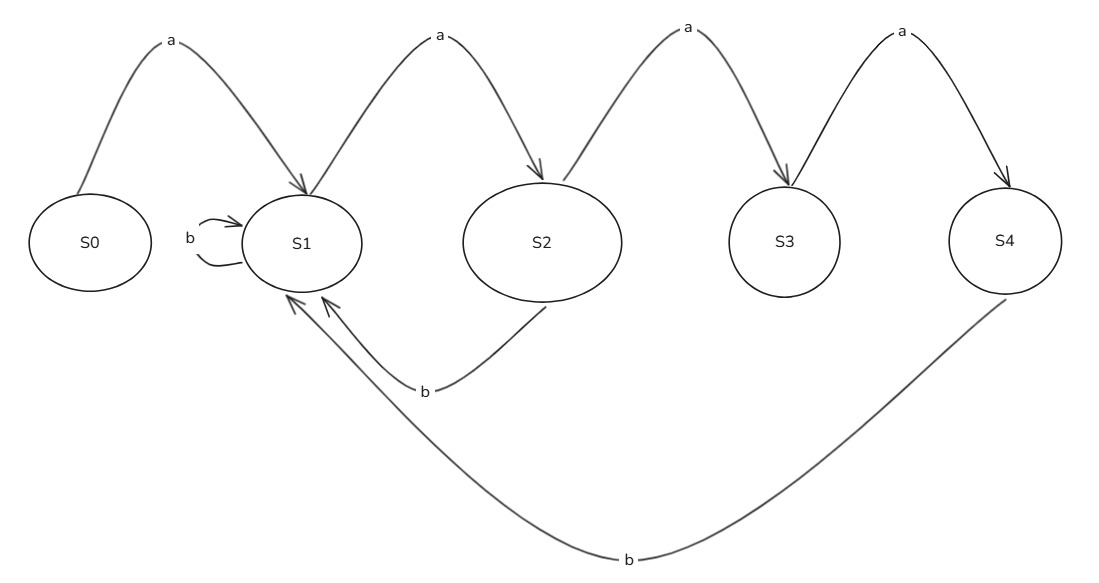
\includegraphics[width=.6\linewidth]{states.jpg}
        \caption{Different States and their Connections}
        \label{Different states}
\end{figure*}

\subsection{Overview of System States} Figure~\ref{Different states} illustrates our finite state machine, implemented
using Aldebaran’s Choregraphe and Python scripts:

\begin{enumerate} \item \textbf{Face Detection (State 0):} NAO scans staff members’ faces and stores in database. After completion, state 1 is triggered.
        \item \textbf{Wave Detection (State 1):} A MediaPipe-based script running in Python continuously scans for a waving hand signal. Upon detection, the system triggers state 2. 
        \item \textbf{Verbal Interaction (State 2):} NAO initiates a spoken dialogue to ask for appointment details. It uses inbuilt speech recognition configured for British English. If the user does not wish to proceed, the system will revert to state 1, ready for the next user. If the user successfully checks in, or they wish to speak to staff, state 3 will be triggered.
        \item \textbf{Email Notification (State 3):} NAO sends an automated email to the relevant staff member. To circumvent network restrictions on SMTP, local testing used a laptop-based hotspot.
        \item \textbf{Feedback Collection (State 4):} NAO requests a brief rating from the user, storing any comments for later review. Once completed, the system returns to state 1.
\end{enumerate}

\subsection{Hardware and Software Setup} Choregraphe runs on a laptop that communicates with the NAO robot over Wi-Fi.
For gestures, a laptop-mounted camera and a Python-based MediaPipe module detect and interpret waving motions.
When network blocks occurred (e.g.\ institutional firewalls), connections were redirected through a personal hotspot to ensure uninterrupted email functionality.

\subsection{Dialogue Capabilities} Choregraphe boxes were primarily used to facilitate dialogue capabilities. Edited \textit{Say} boxes were added to Choregraphe’s \textit{Flow Diagram Panel}, and contained sentences that NAO would say to interact with the user via in-built text-to-speech (TTS) technology. As communication between boxes is event-based, \textit{Say} boxes are triggered onStart and I/O set as “bang”. Naturally, NAO asks the user questions to locate their appointment; therefore, \textit{Say} boxes are primarily followed by Speech Reco. boxes to understand the user’s verbal response. These use an in-built speech-to-text (STT) technology. Each \textit{Speech Reco.} box contains a word list as part of its parameters, these are now words that NAO recognises, and, by utilising a switch case, can respond accordingly to what the user said. \textit{Speech Reco.} boxes have input set to “bang”, output on word recognition set to “string”, and confidence threshold was adjusted to 45% (figure determined during testing). If the confidence threshold was not met, NAO does not recognise the word and will explore contingencies.

A Natural Language Processing (NLP) sentiment detection script was designed but could not be implemented due to integration issues with the NAO robot. This script would have been used for both user inputs and NAO’s verbal outputs. 

\subsection{Person Tracking}
Person tracking capabilities of the NAO receptionist included:
\begin{enumerate}
        \item Face detection and
        \item Wave detection
\end{enumerate}

Face detection was used to detect staff members’ faces and stored on the server database. This facilitated NAO’s capability of announcing the staff’s arrival when they greet the user. Face detection was created using MediaPipe.

Wave detection was implemented to trigger NAO’s verbal interaction with the user. A wave was chosen as a common emblematic non-verbal communication gesture and prevents NAO being active by passersby.  To prompt the user, a sign was placed in front of NAO saying, ‘Wave to speak with the receptionist.’ Wave detection used MediaPipe, specifically using the hand landmark and gesture classification models. 

\subsection{Email Integration} To meet the requirement of the NAO robot being used as a receptionist, a simple email script was designed to run locally on the NAO hardware using a simple mail transfer protocol (SMTP).

\subsection{Code Overview} During the design process, the code was written in Visual Studio (VS) with version control via GitHub, facilitating unit testing in a controlled environment. Once the code was verified and validated, it was integrated into Choregraphe nodes and further tested on a virtual NAO. 

The code was separated across a server and a client. More computationally expensive functions run on the server, whereas simple functions, critical to core functionality, run on NAO. These communicated via a socket framework.

Running gesture recognition and sentiment detection on a server allows deep learning algorithms to benefit from the computing power of the server. This is critical for successful real-time interactions. The server also utilises frameworks that do not integrate well with Python 2 (e.g.  MediaPipe and VADER). Additionally, having these features hosted on a server, multiple NAO robots can utilise these tools and could be extremely useful for clients wishing to purchase and use multiple reception robots.

The remaining code, including TTS, STT, and email functions, runs locally on NAO. It uses minimal computing power and can easily be run in real-time on NAO’s hardware.

\subsection{GitHub} A shared GitHub housed README files, NAO scripts, and LaTeX documentation for report writing. Branches broke down project tasks and features, whilst version control assisted with project collaboration and testing. See Appendix for supporting GitHub documentation.

\subsection{Design Rationale} We opted for a height-aligned placement of NAO to improve authority and user engagement,
as recommended by Rae et al.\cite{Rae2013}. This also aligns with Sutherland et al.\cite{Sutherland2019}, who showed the benefits of
a robotic receptionist in clinical settings. This project expands on their Wizard-of-Oz study by allowing NAO to generate all behaviours without remote operators.

\subsection{Contingency Measures} In practice, user trust decreases sharply when robots show consistent errors, as reported by Bistolfi~\cite{Bistolfi2022}.
Therefore, clear fallback steps were embedded:
\begin{itemize}
        \item If the appointment check-in fails, staff are alerted via email.
\end{itemize}

\subsection{Hazard Mitigation} Following a risk assessment, a highlighted safety concern of NAO are the ‘pinch points’ during robotic movements. To avoid physical contact, NAO will be placed behind a desk and out of reach from the user.

\section{Testing and Results}

TBD

\section{HRI Dialogue Example}

\textit{[User wave detected]}
Gordon: Hi! My name is Gordon. Do you have an appointment?
User: Yes, I do.
Gordon: Who do you have an appointment with?
User: [unrecognisable mumbling]
Gordon: Sorry, didn't catch that.
User: I have an appointment with Bob.
\textit{[Gordon checks the database for an employee called Bob. Bob doesn’t exist.]}
Gordon: May I ask for your confirmation number?
User: My appointment number is 4.
\textit{[Gordon checks the database for a matching confirmation number. Confirmation number exists.]}
Gordon: I have got you.
\textit{[Gordon sends staff member an email]}
Gordon: I have sent an email to the member of staff. Someone will be with you shortly.  In the meantime, how would you rate your experience with me on a scale of 1 to 10?
User: 10! Your service was fantastic.
Gordon: Your feedback is greatly appreciated, thank you. 
\textit{[Gordon detects the staff member walking in]}
Gordon: Our staff is here to help you. Bye.

Scenario: A patient checks in with NAO. The user has an appointment with a staff member, however, that staff member does not exist, NAO prompts the user for their confirmation number. NAO locates the appointment and sends an email to the correct employee. Whilst the user is waiting, NAO asks for user feedback. NAO detects the staff member and announces their arrival.

This scripted scenario highlights two particular failure points anticipated in the system design. Firstly, NAO cannot recognise the user’s first response detailing who they have an appointment with. Secondly, the user mistakenly provides the name of someone who does not work there.  The system is designed to allow a maximum of two attempts to find the employee, then the user is prompted to provide a confirmation number. If the appointment is located, the script follows as above. Alternatively, if the appointment cannot be found, NAO can follow an expanded script asking if the user would like to speak with a human and emails the manager to assist. NAO can determine these failure points as the Python script contains a predetermined list of the employees. NAO listens for these predetermined words. If the user fails to correctly articulate an employee’s name from the predetermined list, NAO will then proceed with the contingencies put in place as part of the system design. To maintain a positive user experience, the user will only be prompted to repeat themselves once, beyond this, human intervention will be offered to avoid user frustrations with the robot. 


\section{Future Work}Facial recognition was planned and developed but was not able to be featured in the final testing due to 
technical difficulties. Future work on this project would include and expand upon this capability as recognising (and potentially 
analysing) individuals vastly increases the functionality and perceived intelligence of the system.

To improve the quality of the current conversations, integrating a more robust NLP algorithm increases the likelihood that the Nao 
robot correctly understands the user’s intent from a single output. Currently, any output outside of expected values is considered 
an error and handled accordingly. NLP allows more unexpected inputs to be parsed for key information that otherwise would’ve been 
missed, directing the robot towards a more appropriate response.

While these improvements would improve the technology, extensive user testing (especially within the intended medical space) is the 
best way to understand the system's shortcomings and improve accordingly.

\section{Discussion}

\subsection{Project Limitations}

\begin{enumerate} \item \textbf{Limited speech recognition.} NAO’s speech recognition can struggle with diverse accents and dialects. Integrating more advanced speech recognition software such as Microsoft Azure can improve this with better accuracy.
        \item \textbf{Restricted physical interaction.} NAO’s limited mobility may offer unrealistic or unidentifiable gestures to its users. To avoid confusions, NAO should maintain basic gestures, and, if required, a video feed on a tablet could supplement NAO’s intentions.
        \item \textbf{Accessibility issues.} Medical environments are subject to users with a diverse range of accessibility needs. The NAO robot required a user to see a sign, prompting the user to wave and initiate communication with the robot. If a user has sight impairments, NAO would not successfully check-in the user.  Advanced image recognition could be used to detect visual aids such as guide dogs or mobility canes. Upon detection, NAO could automatically be triggered into state 2, proceeding with checking-in. To build upon the robust nature of NAO in an environment with accessibility needs, a mitigation plan for each ailment could be developed along with supporting improvements to assist these users.
        \item \textbf{User acceptance and usability.} Older users may be uncomfortable interacting with robots and may find NAO confusing or intimidating. Providing visible instructions and support materials such as posters could encourage familiarity and engagement.
\end{enumerate}


\subsection{Module Feedback} The HRI module was both interesting and highly engaging. It achieved an excellent balance between critical theoretical knowledge on HRI system architectures and practical application using the NAO robot. The module’s emphasis on user-centred design and enhancing the overall user experience is an important skill to create successful projects.

A standout highlight was the BRL visit, which offered invaluable exposure to real-world applications of HRI technologies and reinforced the theoretical concepts covered in the module.

One potential improvement would be to increase contact time with the NAO robot, either through a loan system or extended lab sessions. This would allow students to spend more time experimenting with programming and troubleshooting fostering deeper learning and confidence for the assessment.



\section{Conclusion}

TBD

\bibliographystyle{plain}
\bibliography{references}

\end{document}
